\documentclass[ti]{texufpel} %use tid para doutorado e ti para mestrado

\usepackage[utf8]{inputenc} % acentuacao
\usepackage{graphicx} % para inserir figuras
\usepackage[T1]{fontenc}
\usepackage{subfigure}
\usepackage{todo}
\usepackage{amssymb}

\hypersetup{
    hidelinks, % Remove coloração e caixas
    unicode=true,   %Permite acentuação no bookmark
    linktoc=all %Habilita link no nome e página do sumário
}

\unidade{Centro de Desenvolvimento Tecnológico}
\programa{Programa de Pós-Graduação em Computação}
\curso{Ciência da Computação}

\title{Memórias Transacionais}

\author{Costa}{Michael Alexandre}
\advisor[Prof.~Dr.]{Du Bois}{André Rauber}
\coadvisor[Prof.~Dr.]{Pilla}{Mauricio Lima}

%Palavras-chave em PT_BR
\keyword{Memótia Transacional}
\keyword{NUMA}
\keyword{UMA}
\keyword{Escalonamento}

%Palavras-chave em EN_US
\keywordeng{Transacional Memory}
\keywordeng{NUMA}
\keywordeng{UMA}
\keywordeng{Scheduler}

\begin{document}


\maketitle

\sloppy

%Resumo em Portugues (no maximo 500 palavras)
\begin{abstract}
  ...
\end{abstract}

\begin{englishabstract}%
  {Transacional Memory}% {Titulo do Trabalho em Ingles}

  ...
\end{englishabstract}

%Lista de Figuras
\listoffigures

%Lista de Tabelas
\listoftables

%lista de abreviaturas e siglas
\begin{listofabbrv}{SPMD}
        \item[ATS] Adaptive Transactional Scheduling
        \item[STM] Software Transactional Memory
        \item[TM] Transactional Memory
        \item[NUMA] Non-Uniform Memory Access
        \item[UMA] Uniform Memory Access
\end{listofabbrv}

\tableofcontents

\chapter{Introdução}

As arquiteturas paralelas são praticamente onipresentes nas plataformas computacionais modernas. Processadores convencionais com múltiplos núcleos são usados para construção de computadores domésticos e supercomputadores. O paralelismo desses processadores tendem a crescer com o passar dos anos, pois o aumento de desempenho dos computadores atuais tem se baseado no desenvolvimento de arquiteturas paralelas.

Para que as aplicações possam extrair o melhor desempenho das arquiteturas paralelas, o código deve explorar ao máximo o poder computacional oferecido pelas diversas unidades de processamento, porém, a programação paralela está longe de ser uma atividade trivial. O acesso à memória compartilhada é um dos cuidados que programadores devem tomar ao desenvolver aplicativos para máquinas multi-core, para isto, as linguagens fornecem mecanismos de sincronização como \emph{locks} e \emph{mutex}, este modelo de programação é difícil e propenso a erros. Visando reduzir a dificuldade no desenvolvimento de programas confiáveis para este tipo de máquina, tem se como alternativa o uso de Memórias Transacionais.

Memórias Transacionais~(TM) são mecanismos de sincronização que realizam execuções atômicas e isoladas de partes compartilhadas do código. Na programação utilizando \emph{Software Transactional Memory}~(STM), o acesso à memória compartilhada é realizado dentro de uma transação executada atomicamente~\cite{teixeira15}. A programação com STM permite que o programador não se preocupe com as aquisições e liberações de \emph{locks}, este deverá delimitar apenas as seções críticas, o que facilita a programação.

As arquiteturas \emph{NUMA} (\emph{Non-Uniform Memory Access}) surgiram como alternativa às limitações de escalabilidade sofridas pelas arquiteturas \emph{UMA} (\emph{Uniform Memory Access}). As arquiteturas \emph{NUMA} possuem múltiplos processadores, compostos por vários núcleos e blocos de memória dedicados, a sua principal característica é o custo de tempo diferente para o acesso à memória~\cite{rodolfo14}.

Com o aumento do paralelismo existente nas arquiteturas atuais há um aumento no número de contenção, ocasionando conflitos e \emph{aborts} nas STMs. Estudos de STM buscam utilizar escalonadores para reduzir o número de conflitos e otimizar tempo de execução. Porém ao estudos recentes de escalonadores de STM tem como foco apenas arquiteturas UMA.

Este trabalho apresenta os principais trabalhos relacionado a escalonadores de STM com base nas categorias apresentadas em \cite{sanzo17}. Este trabalho realizou um estudo sobre os escalonadores de STM com foco de determinar as atuais heurísticas utilizadas em STM, assim como revisou as principais característica de arquiteturas UMA e NUMA.

\chapter{Memória Transacional}

Memória Transacional, ou \emph{Transactional Memory}~(TM), é uma classe de mecanismos de sincronização que fornece uma execução atômica e isolada de alterações em um conjunto de dados compartilhados. Estas estão sendo desenvolvidas para que no futuro tornem-se o principal meio de fazer a sincronização em um programa concorrente, substituindo a sincronização baseada em \emph{locks}~\cite{herlihy06}. As TMs podem ser implementadas em \emph{software} (STM), em \emph{hardware} (HTM) ou ainda em uma versão híbrida de \emph{hardware} e \emph{software}.

Na programação utilizando STMs, todo o acesso à memória compartilhada é realizado dentro de transações e todas as transações são executadas atomicamente em relação a transações concorrentes.

A principal vantagem na programação usando STM é que o programador apenas delimita as seções criticas e não é necessário preocupar-se com a aquisição e liberação de \emph{locks}. Os \emph{locks}, quando utilizados de forma incorreta, podem levar a problemas como \emph{deadlocks}~\cite{bandeira10}.

\section{Propriedades}

Transação é uma sequência finita de escritas e leituras na memória executada por uma \emph{thread}~\cite{herlihy93}, e deve satisfazer três propriedades:

\begin{itemize}
 \item \textbf{Atomicidade}: cada transação faz uma sequência de mudanças provisórias na memória compartilhada. Quando a transação é concluída, pode ocorrer um \emph{commit}, tornando suas mudanças visíveis a outras \emph{threads} instantaneamente, ou pode ocorrer um \emph{abort}, fazendo com que suas alterações sejam descartadas;

 \item \textbf{Consistência}: as transações devem garantir que um sistema consistente deve ser mantido consistente. Esta propriedade esta relacionada com o conceito de invariância;

 \item \textbf{Isolamento}: as transações não interferem nas execuções de outras transações, assim parecendo que elas são executadas serialmente. Uma transação não observa o estado intermediário de outra.
\end{itemize}

\section{Versionamento de Dados}

O versionamento de dados faz é responsável pelo gerenciamento das versões dos dados. Ele armazena tanto o valor do dado no início de uma transação como também o valor do dado modificado durante a transação, isso para garantir a propriedade de atomicidade~\cite{baldassinTese09}.

\begin{figure}[!htp]
\centering
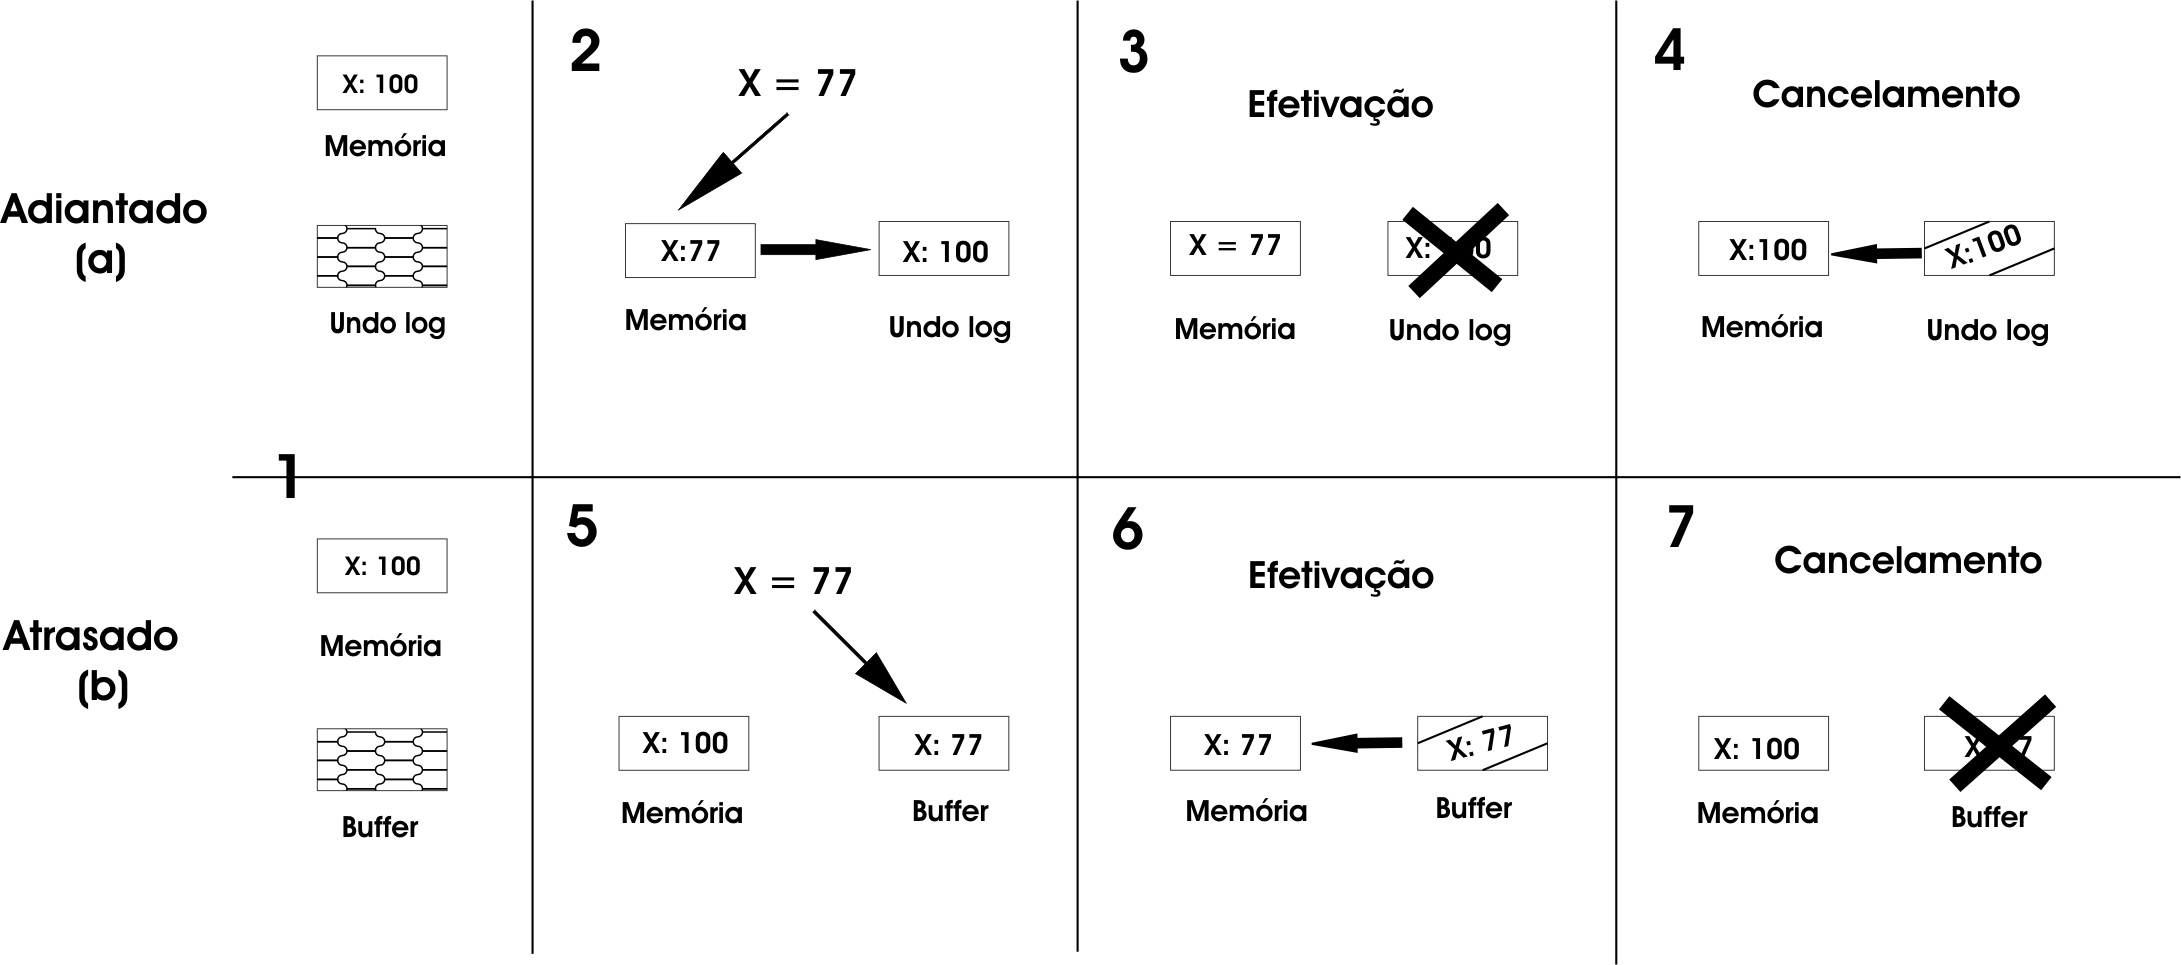
\includegraphics[height=7cm]{Imagens/versionamento.png}
\caption{Exemplo de versionamento adiantado (a) e atrasado (b). Fonte:~\cite{baldassinTese09}}
\label{figuraVersionamento}
\end{figure}

Existem dois tipos de versionamento de dados:

\begin{itemize}
 \item \textbf{Versionamento Adiantado}: como pode ser visto na Figura~\ref{figuraVersionamento}~(a), o valor modificado durante a transação é armazenado direto na memória e o valor inicial é armazenado em um \emph{undo log}, para que no caso de cancelamento na transação o valor inicial seja restaurado na memória.

 \item \textbf{Versionamento Atrasado}: como pode ser visto na Figura~\ref{figuraVersionamento}~(b) neste versionamento o valor modificado durante a transação é armazenado em um \emph{buffer} e o valor inicial é mantido na memória até que aconteça um \emph{commit} na transação, onde o valor armazenado no \emph{buffer} é escrito na memória. Caso aconteça o cancelamento na transação, o valor do \emph{buffer} é descartado.
\end{itemize}

\section{Detecção de Conflito}

Mecanismos de detecção de conflitos verificam a existência de operações conflitantes durante uma transação. Um conflito ocorre quando duas transações estão acessando um mesmo dado na memória e pelo menos uma das transações está fazendo uma operação de escrita~\cite{baldassinTese09}.

Da mesma forma que o versionamento de dados, a detecção de conflito também pode ser de dois tipos:

\begin{itemize}
 \item \textbf{Detecção de Conflitos Adiantado}: ocorrem no momento em que duas transações acessam um mesmo dado e uma delas faz uma operação de escrita. Essa operação de escrita é detectada e então uma transação é abortada. Neste tipo de detecção pode ocorrer o problema chamado de \emph{livelock}, quando duas transações ficam cancelando-se, desta forma, a execução do programa não progride. A Figura~\ref{figuradeteccaoadiantado} mostra como é feita a detecção de conflitos adiantado.

 O Caso~1, mostra a execução sem conflitos, onde as duas transações são executadas sem problemas. Já o Caso~2, mostra o que acontece quando ocorre um conflito, onde T1 lê A e logo depois T2 escreve em A, então o conflito é detectado e T1 é abortada, após ser efetivada T2, a transação T1 consegue ler A sem problema de conflito. Por fim o Caso~3 mostra a situação de \emph{livelock}, onde as duas transações tentam ler e escrever em A, assim as duas acabam sempre se abortando.

\begin{figure}[!htp]
\centering
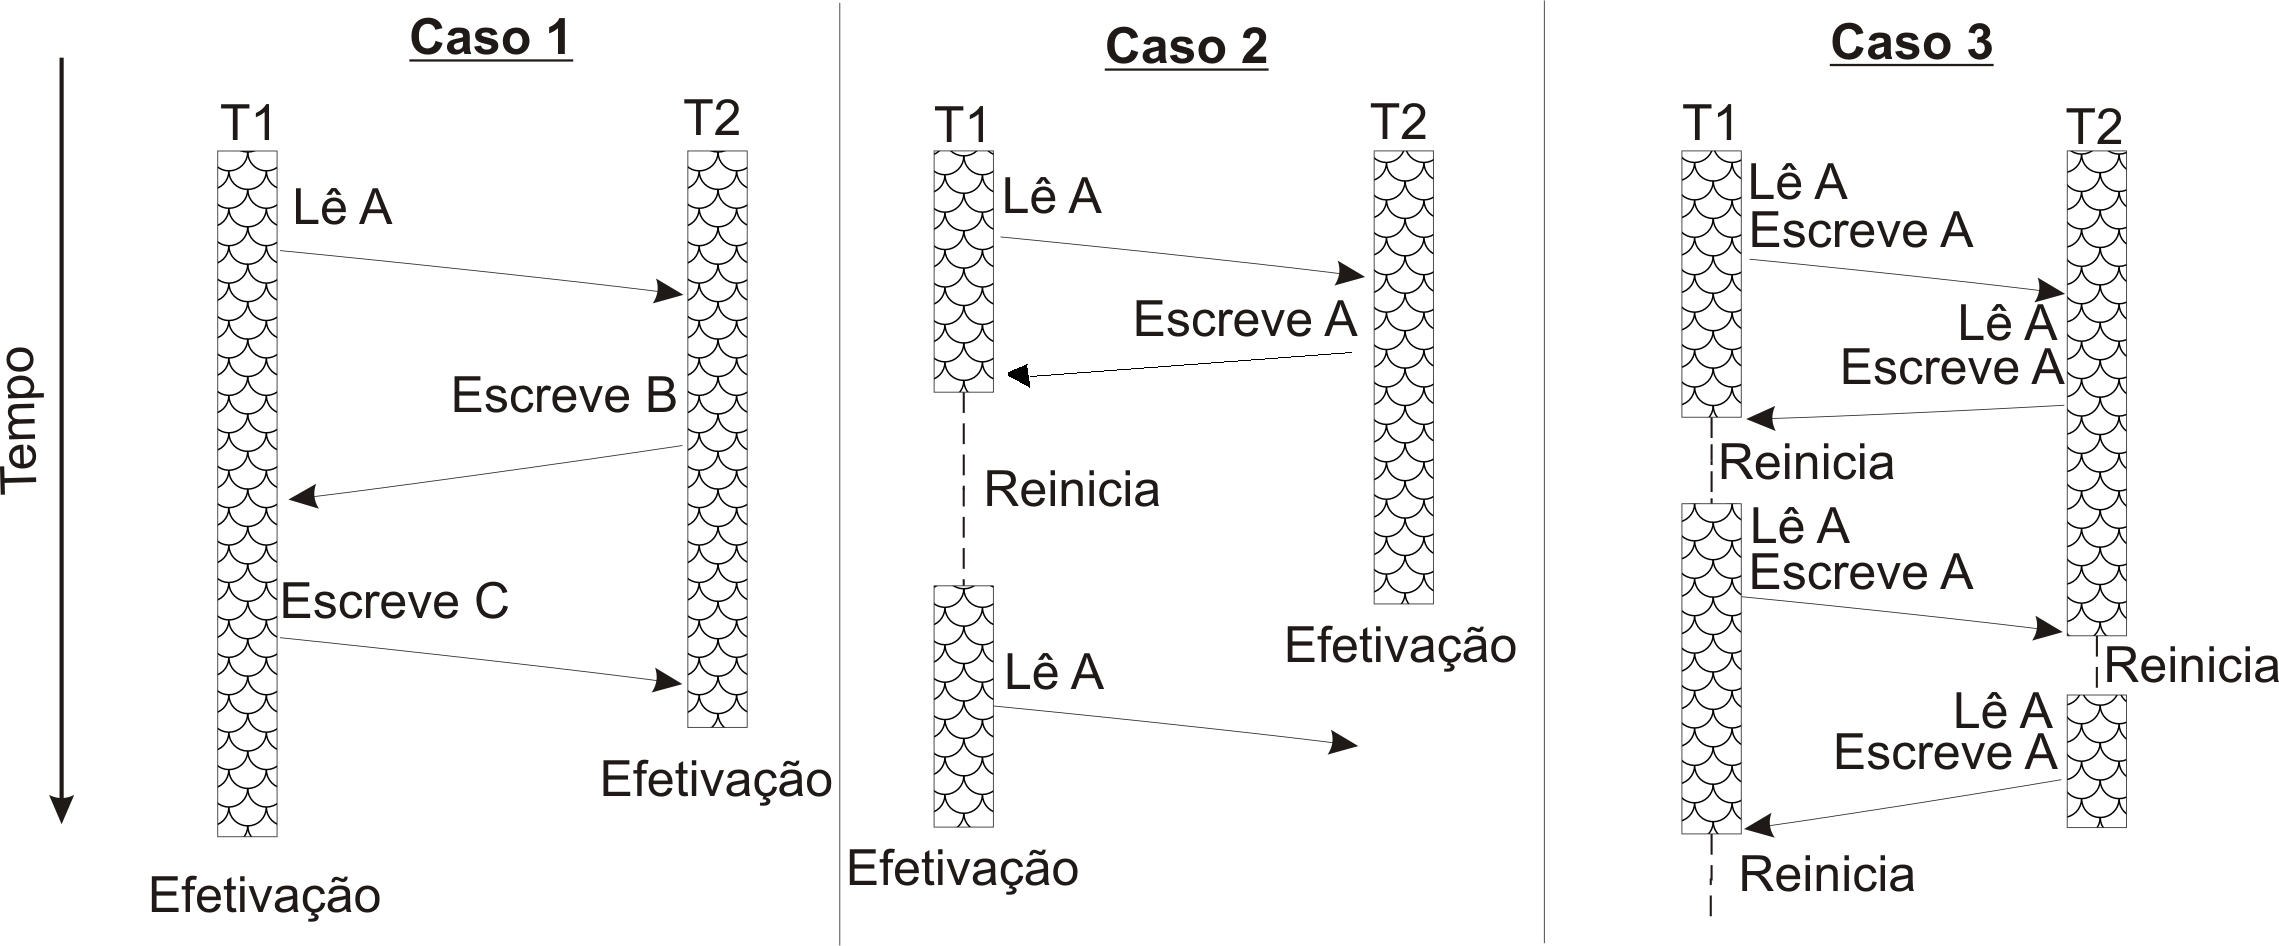
\includegraphics[height=6.5cm]{Imagens/conflitoadiantado.png}
\caption{Detecção de conflitos em modo adiantado. Fonte:~\cite{rigo07}}
\label{figuradeteccaoadiantado}
\end{figure}

 \item \textbf{Detecção de Conflitos Atrasado}: Este tipo de detecção de conflito ocorre no final da transação.  Antes da transação ser efetuada, é verificado se ocorreu um conflito. Caso tenha ocorrido, a transação é cancelada, senão é efetivada. Para transações muito grandes não é recomendado este tipo de detecção, pois uma transação grande pode ser abortada várias vezes por transações pequenas, assim gastando tempo de processamento desnecessário, este problema se chama \emph{starvation}. A Figura~\ref{figuradeteccaoatrasado} mostra como é feita a detecção de conflitos atrasado.

 O Caso~1, mostra as transações acessando dados diferentes, não ocasionando conflitos. No Caso~2, T2 lê A que é escrita por T1. A T2 só nota o conflito quando T1 é efetivado. Logo depois de notar o conflito T2 é abortada. No Caso~3 não ocorre nenhum conflito, pois T1 lê A antes de T2 escrever. O Caso~4 mostra a situação em que, após ser cancelada, T1 volta a executar.
\end{itemize}

\begin{figure}[!htp]
\centering
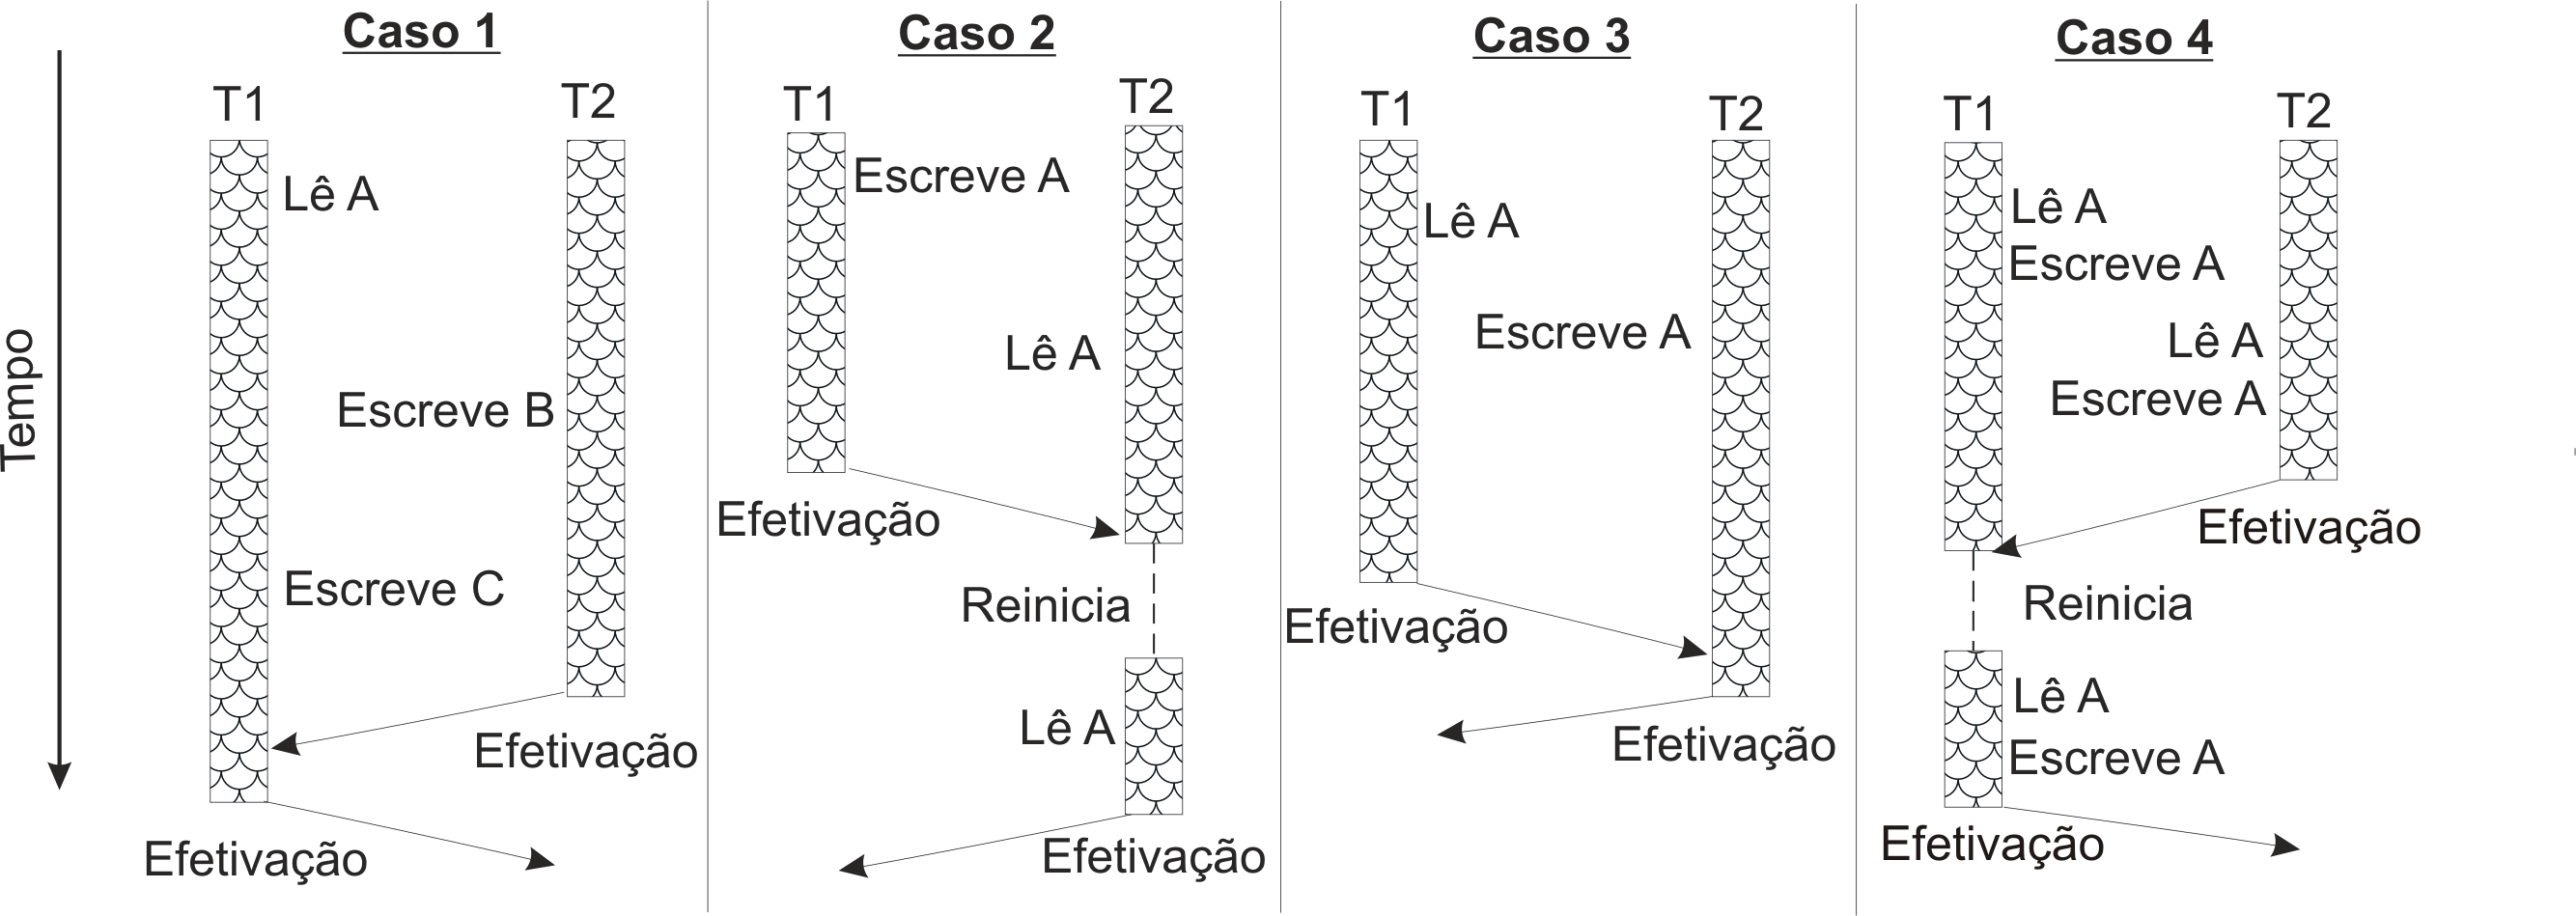
\includegraphics[height=6.5cm]{Imagens/conflitoatrasado.png}
\caption{Detecção de conflitos em modo atrasado. Fonte:~\cite{rigo07}}
\label{figuradeteccaoatrasado}
\end{figure}

Para solucionar o problema de qual transação continuará executando, quando ocorre um conflito, é utilizado um gerenciador de contenção~\cite{harris10}. O gerenciador de contenção é o responsável por decidir quando e qual transação vai ser abortada, isso para garantir que a execução do programa prossiga sem problemas.

\chapter{Escalonamento de STM}

  A bibliografia de STM apresenta um gama distinta e extensa de estratégias de escalonamento. Estas diferem-se devido as distintas características de aplicações encontradas. Nas quais podem apresentar maior ou menor nível de contenção, diferentes read-sets e write-sets, entre outras características.

  Os algoritmos de escalonamento visam otimizar o tempo de execução. Para isto devem inserir o menor \emph{overhead} possível no código propondo uma estratégia eficiente para as características do problema abordado. Alguns algoritmos estudados, como \emph{CAR-STM}~\cite{dolev08}, buscam serializar transações conflitantes com a utilização de filas de transações.

  Os escalonadores de STM estudados na bibliografia caracterizam-se por executar o escalonamento em dois níveis distintos. Os dois níveis buscam reduzir o tempo de execução e garantir a execução do programa. Estes escalonamentos de STM são o escalonamento de \emph{threads} e de transações.

  O escalonamento de \emph{threads}, busca executar sua tomada de decisão sobre as \emph{threads} ativas no programa, podendo adicionar mais \emph{threads}, remove-las, ou migra-las entre os \emph{cores}.

  O escalonamento de transações, busca executar sua tomada de decisão sobre as transações do programa, estas podem estar em execução, já terem sido abortadas, ou serem a próxima a executar.

  As tomadas de decisões dos escalonadores citados acima se dá a partir de outras características. Estas avaliam de forma diferente os dados para a tomada de decisão e em tempos de execução diferentes, assim como, podem efetuar operações distintas conforme suas premissas de escalonamento.

\section{Características e Técnicas}

O trabalho \cite{sanzo17}, classifica as técnicas de escalonamento de STM como, baseadas em heurísticas e baseadas em modelos, esta classificação é apresentada na Figura~\ref{figuraCategoria}, onde cada classe, apresenta técnicas distintas de escalonamento.

Estas diferentes técnicas apresentadas foram exploradas e exemplificadas no trabalho citado acima. As subseções a seguir vão abordar e detalhar estas técnicas, assim como seus algoritmos.

\begin{figure}[!htp]
\centering
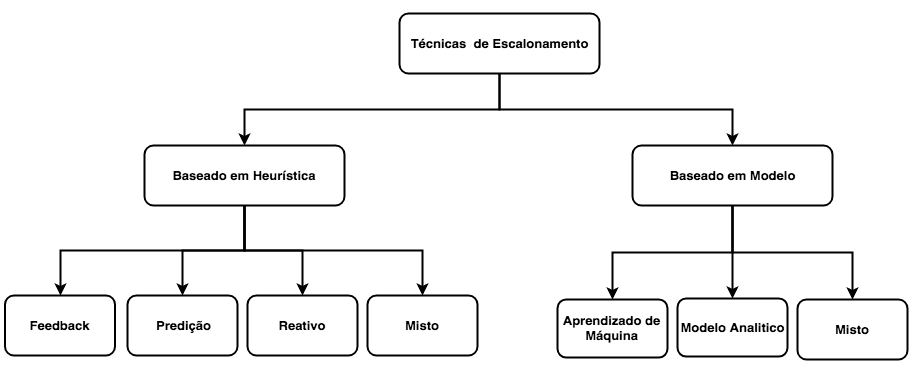
\includegraphics[height=6.5cm]{Imagens/categoriasEscalonamento.png}
\caption{Classificação das técnicas de escalonamento. Fonte:~\cite{sanzo17}}
\label{figuraCategoria}
\end{figure}

\subsection{Técnica baseada em Feedback}

As técnicas baseadas em feedback utilizam um sistema de loop fechado para controle de um sistema dinâmico. Essa técnica utiliza um parâmetro de desempenho que é avaliado pelo escalonador a cada iteração do loop para decidir a ação a ser executada, um exemplo de escalonador baseado em feedback é denominado \emph{Adaptive Transactional Scheduling} (ATS).

O escalonador ATS, apresentado em \cite{yoo08}, tem como objetivo otimizar a execução de código e reduzir o número de conflitos por meio da serialização das transações conflitantes. Para serializar as transações o escalonador utiliza uma fila de compartilhamento global.

O escalonador toma a decisão de serializar ou não uma transação conflitante utilizando um parâmetro de feedback denominado \emph{Contention Intensity} (CI). Cada \emph{thread} em execução possui um CI, que é calculado individualmente por uma média dinâmica, este cálculo é efetuado quando uma transação é anulada ou confirmada. A função que calcula o CI é: $CI = \alpha * CIprev + (1 - \alpha) * CC$.

Onde $CIprev$ é o valor anterior a $CI$, $CC$ é igual a 0 se a transação for anulada e igual a 1 se a transação for confirmada, $\alpha$ possui um valor entre 0 e 1, e afeta o peso histórico das transações do \emph{thread}.

Quando um $CI$ ultrapassa o limite previamente definido, o escalonador toma a decisão de serializar as transações executadas por este \emph{thread} em relação às transações executadas por outro \emph{thread}, inserindo então as transações na fila de compartilhamento global.


\subsection{Técnica baseada em Previsão}

As técnicas baseadas em previsão utilizam probabilidade para tomar a decisão apropriada para sua execução. Essa técnica utiliza um conjunto de dados de um mesmo parâmetro para estimar a probabilidade de execução, assim o escalonador toma a decisão de execução dinamicamente. Um exemplo de escalonador baseado em previsão é denominado \emph{Shrink}.

O escalonador \emph{Shrink}, apresentado em \cite{dragojevic09}, utiliza a suposição de localidade temporal e serializa as transações se os conjuntos de dados previstos mostrarem que um conflito pode ocorrer.

Para isto, é utilizado como base, os dados lidos pelas n transações executadas por um \emph{thread}. Este conjunto de leitura de uma transação utiliza o valor n como uma janela de localidade.

Assim, se um item de dados tiver sido lido pela transação anterior, é incrementado, com uma constante de confiança (CI), o parâmetro confiança (C). Se este ultrapassar o limite de confiança estipulado, o item de dados é adicionado ao conjunto de leitura previsto.

O conjunto de gravação é previsto apenas para reiniciar as transações, presumindo-se que este inclua dados pertencentes ao conjunto de gravação da última transação anulada.

Visando reduzir o \emph{overhead} de execução, o escalonador \emph{Shrink} entra em ação para um \emph{thread} apenas quando sua taxa de sucesso de transação está abaixo de um limite de sucesso.


\subsection{Técnicas Reativas}

As técnicas reativas adotam uma estratégia onde o escalonador entra em ação após uma transação ser abortada, isso busca evitar conflitos repetidos. Esta estratégia baseia-se na suposição de que os dados acessados por uma transação abortada tem a possibilidade de serem os mesmos acessados durante sua reexecução, ocasionando novo conflito com a transação ainda em execução. Um exemplo de escalonador que utiliza técnicas reativas é conhecido como \emph{CAR-STM}.

O escalonador \emph{CAR-STM}, apresentado em \cite{dolev08}, apresenta duas políticas. A primeira, denominada \emph{Basic Seraling Contention Management}~(DSCM), reduz a probabilidade de duas transações, que já conflitaram, conflitem novamente. A segunda política, denominada \emph{Gerenciamento de Prevenção de Serialização Permanente}~(PSCM), garante que duas transações conflitantes nunca conflitem novamente.

Com a política PSCM, se uma transação \emph{A} entrar em conflito com uma transação \emph{B} e \emph{A} for iniciada após \emph{B}, \emph{A} será abortada. A transação abortada é colocada na fila de execução da \emph{thread} na qual a transação conflitante pertence. Isso reduz a probabilidade de ocorrer novamente um conflito entre estas transações.

Ainda há a possibilidade de ocorrer um conflito entre estas transações. Se \emph{B} conflitar com uma terceira transação, então \emph{B} será colocada em uma fila de transação que será executado por outro \emph{thread}, assim, permitindo novamente um conflito com \emph{A}. Para evitar esta situação, a política PSCM, marca transação abortada como subordinada a transação conflitante, assim, caso a transação conflitante for movida de fila, as transações subordinadas a esta serão movidas junto.

O \emph{CAR-STM} também possui a opção de escalonamento proativo, onde o escalonador não precisa que um conflito ocorra. Neste caso, o escalonador possui informações sobre a possibilidade de conflito entre pares de transações. Estas informações são fornecidas ao escalonador pela aplicação utilizada, deixando a cargo do desenvolver a tarefa de manter o escalonador ciente dos acessos realizados pelas transações.

\subsection{Técnica baseada em Heurística Mista}

As técnicas baseadas em heurísticas mista buscam mesclar as diferentes técnicas comentadas acima, para tirar proveito de diferentes perfis de transações. Assim, o escalonador pode tomar a melhor decisão de execução de acordo com o perfil de execução das transações.  Um exemplo de escalonador que utiliza técnicas reativas é conhecido como \emph{LUTS}.

O escalonador \emph{Lightweight User-Transaction Scheduler}~(LUTS), apresentado em \cite{nicacio13}, permite a modificação de sua estratégia de escalonamento de forma dinâmica, para isto, este avalia a duração das transações. O \emph{LUTS} utiliza um conjunto de \emph{threads}, com tamanho igual ao número de núcleos disponivel na arquitetura em que será utilizado.

As transações são agrupadas por \emph{IDs}, onde, todas as transações geradas pelo mesmo bloco de código possuem o mesmo \emph{ID}. O escalonador utiliza o tempo médio das últimas 100 transações confirmadas. Se o tempo médio estiver abaixo de um limite de tempo pré definido, o escalonador serializa as transações com base na intensidade de contenção, assim como feito no escalonador ATS. Porém, o LUTS mantém o valor de \emph{IC} por \emph{ID} de transação.

Quando a média de transações está acima do limite, o escalonador armazena a probabilidade de conflito para cada \emph{ID} de transação em uma estrutura de dados. Quando uma \emph{thread} fica disponível, o escalonador lê os \emph{IDs} de todas as transações em execução e as informações das estruturas de dados para selecionar a transação com menor probabilidade de conflito. A probabilidade de conflito de um ID é incrementada quando uma transação confirmada e decrementada toda vez que uma transação for abortada.

\subsection{Técnicas baseadas em Aprendizado de Máquina}

As técnicas baseadas em aprendizado de máquina utilizam modelos de desempenho. A partir de um conjunto de dados que representa o perfil das transações, o algoritmo aplica monta uma rede de aprendizado para formular as relações do modelo de desempenho. Assim, o escalonador utiliza o modelo de desempenho como função de entrada para tomada de decisão. Um exemplo de escalonador baseado em aprendizado de máquina é conhecido como \emph{SAC-STM}.

O escalonador \emph{Self-Adjusting Concurrency STM}~(SAC-STM), apresentado em \cite{rughetti12}, utiliza Rede Neural Artificial (RNA) para gerar modelos de desempenho que serão usados em sua tomada de decisão. Uma RNA é um modelo de aprendizado de máquina que permite aproximar uma função por meio de um processo de treinamento. É utilizado o RNA para estimar o tempo médio de transações por meio de uma função de perfil, utilizando carga de trabalho e número de \emph{threads} simultâneas.

Em tempo de execução, o escalonador executa um \emph{loop} contínuo para regular o número de \emph{threads} ativos. Para cada etapa do \emph{loop} são executadas as seguintes ações:

\begin{enumerate}
 \item Coleta as amostras de carga de trabalho nas últimas n transações;
 \item Utiliza a RNA para estimar os tempos esperados de transação em variação de k para k<=M, onde, k é o recurso de entrada e M é o número de \emph{threads};
 \item Calcula com base nos tempos esperados o rendimento esperado na variação de k;
 \item Mantém k0 \emph{threads} ativos, onde k0 é o número de \emph{threads} para os quais a taxa de transferência é estimada como mais alta.
\end{enumerate}

\subsection{Técnicas Baseada em Modelos Analíticos}

As técnicas baseadas em modelos analíticos utilizam modelos construídos por equações matemáticas para tomada de decisão do escalonador. Assim, esta técnica tem como entrada de uma função analitica a base de dados da transação, na qual a saída da função será utilizada para moldar o modelo utilizado. Um exemplo de escalonador baseado em modelo  analítico é denominado \emph{CSR-STM}.

O escalonador \emph{Concurrency Self-Regulating }~(CSR-STM), apresentado em \cite{sanzo13}, utiliza uma técnica analítica baseada em modelo, onde, o esquema básico de escalonamento é semelhante ao visto no \emph{SAC-STM}. Assim, o número de \emph{threads} ativos é regulado com base no rendimento da aplicação.

O CSR-STM ao contrário do SAC-STM não utiliza RNA, porém, utiliza um modelo de desempenho analítico para estimar a probabilidade de conflitos da transação. Este modelo analitico pode ser personalizado de acordo com aplicação e especificação da máquina utilizada.

\subsection{Técnica baseada em Modelos Mistos}

As técnicas baseadas em modelos mistos buscam mesclar as técnicas baseadas em modelo já apresentadas. Essa técnica busca avaliar o comportamento das transações previamente e utilizar estratégias mistas para criar o melhor modelo para o escalonador tomar suas decisões. Um exemplo de escalonador baseado em modelo  misto é o \emph{AML}.

O escalonador \emph{Analytical/Machine Learning}~(AML), apresentado em \cite{rughetti14}, é baseado em modelos mistos que usa o modelo analítico visto em CSR-STM e o aprendizado de máquina visto em SAC-STM. O escalonador busca obter o melhor dos dois modelos, assim, utiliza a fase leve de perfil da carga de trabalho do modelo analitico e a estimatica de alto desempenho das RNAs.

O escalonador utiliza o modelo analítico para gerar amostras virtuais que cobrem um subconjunto do domínio dos recursos de entrada. Em seguida, é gerado um único conjunto de dados com amostras reais e virtuais, este conjunto é utilizado para treinar a RNA. Com isto, o escalonador então obtém estimativas de desempenho mais confiáveis para tomada de decisão.

\chapter{Arquiteturas NUMA e UMA}

Dependendo da localização física da memória em relação aos processadores, o tempo de acesso a uma posição de memória pode ser uniforme ou não. Surge então as arquiteturas denominadas de \emph{UMA~(Uniform Memory Access)} e \emph{NUMA~(Non Uniform Memory Access)} \cite{carissimi07}.

Máquinas \emph{NUMA} possui a vantagem de agregar maior paralelismo ao adicionar mais processadores sem aumentar o número de conflitos e o gargalo de acesso ao barramento. Sua arquitetura é feita para que os processadores não utilizem o mesmo barramento de acesso à memória como é feito em arquiteturas \emph{UMA}.

As arquiteturas \emph{NUMA} possuem múltiplos núcleos dispostos em conjuntos de processadores (Nodos), a memória é fisicamente composta por vários bancos de memória, podendo estar cada um deles vinculados a um Nodo e a um espaço de endereçamento compartilhado. Nesse caso, quando o processador acessa à memória que está vinculada a si, diz-se que houve um acesso local. Se o acesso for à memória de outro processador, diz-se que ocorreu um acesso remoto.

Os acessos remotos são mais lentos que os acessos locais, uma vez que é necessário passar pela rede de interconexão para que se consiga chegar ao dado localizado na memória remota \cite{rodolfo14}. A Figura~\ref{arquiteturas_config} ilustra de maneira genérica, \ref{uma_fig} uma máquina de arquitetura \emph{UMA} e \ref{numa_fig} uma máquina de arquitetura \emph{NUMA}. Pode-se observar que, na arquitetura \emph{UMA} representada na Figura~\ref{uma_fig}, às operações relacionadas à memória (leituras e escritas), independente da unidade de processamento \emph{(P0, P1, ..., Pn)} que estão partindo, possuem o mesmo tempo de acesso, pois todos acessam a memória utilizando o mesmo caminho.

Já na Figura~\ref{numa_fig}, existem dois possíveis e distintos caminhos para acessar à memória, dependendo de qual unidade de processamento irá partir o acesso e da localização física da memória a ser acessada: (i) Acesso Local (\emph{P2} acessando à memória \emph{M2}) e (ii) Acesso Remoto (\emph{P2} acessando à memória \emph{M1}). Os tempos de acessos à memória local de um processador, tanto para leitura quanto para escrita de dados e instruções, são menores do que os tempos de acessos às memórias remotas. Neste tipo de arquitetura, os acessos a memória ocorrem de maneira não uniforme, essas assimetrias no acesso caracterizam este tipo de arquitetura.

\begin{figure}[!htp]
\centering
\subfigure[Arquitetura UMA]{
 \label{uma_fig}
 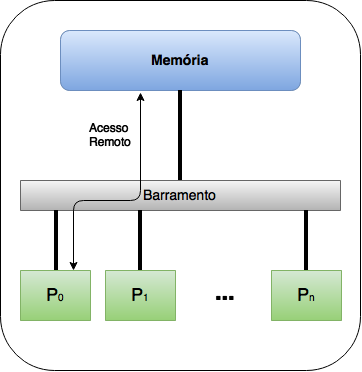
\includegraphics[height=6cm]{Imagens/UMA.png}
}
\subfigure[Arquitetura NUMA]{
 \label{numa_fig}
 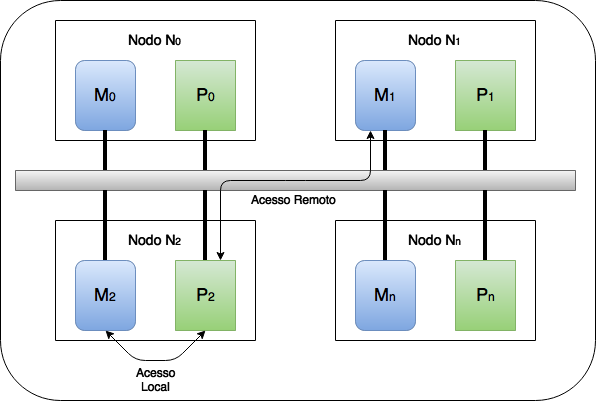
\includegraphics[height=6cm]{Imagens/NUMA.png}
}
\caption{Configuração das arquiteturas UMA e NUMA. Fonte:~\cite{rodolfo14}}
\label{arquiteturas_config}
\end{figure}

O custo não uniforme de acesso à memória é importante para o desempenho de uma aplicação, pois este pode oferecer desvantagens quando não forem avaliados. Uma forma bastante comum de medir a não uniformidade de acessos à memória nas arquiteturas assimétricas, é considerar a razão entre o acesso a uma posição de memória remota e um acesso a uma posição de memória local. Esta razão é denominada fator \emph{NUMA}, uma máquina pode apresentar diferentes valores para o fator \emph{NUMA}, dependendo de quais memórias serão acessadas pelos processadores. Portanto, para que uma aplicação execute de forma eficiente é desejável que os processos sejam escalonados próximos a faixa de endereçamento que eles acessam, assim reduzindo o fator \emph{NUMA}.

É importante conhecer as características da arquitetura \emph{NUMA}, principalmente a latência de acesso às memórias remotas. Estas informações servem de subsídio ao desenvolvedor para que este consiga definir estratégias de escalonamento de tarefas mais eficientes para aplicações que executam neste tipo de arquitetura.

\chapter{Discussões}

Os artigos revisados neste trabalho apresentam diferentes formas de escalonamentos voltados a memórias transacionais com foco na redução de conflitos e otimização de desempenho. Estes algoritmos abordam técnicas com características distintas nas tomadas de decisão, porém, todos são voltados para o uso de STM em arquiteturas UMA.

Os trabalhos descritos mesclam diferentes abordagens para diminuir conflitos, desde avaliar o histórico de transação a utilização de aprendizado de máquina para aproximar a melhor curva de execução de STM, assim, é possível por meio do escalonador tomar decisões como serializar transações conflitantes, utilizar mais ou menos threads simultâneas ou acordar a transação com menor probabilidade de conflito.

Estas característica maximizam a execução de transações em arquiteturas UMA, para a qual os algoritmos de STMs foram projetados. Mas não consideram o uso de STMs em arquiteturas NUMA, desta forma não consideram o conceito do fator NUMA, onde a latência de acesso a memória pode causar overhead acima do esperado em uma execução.

Este trabalho apresentou uma visão atual sobre os principais trabalhos relacionados a escalonadores de STMs, utilizando a divisão de técnicas vista no trabalho \cite{sanzo17}. Este trabalho permite avaliar as metodologias já propostas de escalonamento STM para mensurar qual a melhor abordagem a ser utilizada em trabalhos futuros.

\chapter{Conclusão}

O trabalho teve como objetivo principal revisar as principais técnicas de escalonadores STM atuais. Também foram revisados os conceitos de memórias transacionais e arquiteturas UMA e NUMA. Com isto, podemos avaliar abordagens já realizadas para reproduzir e comparar em diferentes arquiteturas.

As técnicas revisadas e descritas são desenvolvidas para o uso de STMs em arquiteturas UMA. Estas visam tirar o melhor proveito de STM e otimizar a execução, reduzindo conflitos e distribuindo de maneira eficiente a carga de trabalho. Este objetivo pode ser obtido com uso de técnicas distintas, onde, algumas mesclam recursos para tirar otimizar os escalonadores.

Estas técnicas são voltadas para a arquitetura UMA, e portanto, não consideram as latências de acesso a memória e não apresentam seu desempenho perante estas arquiteturas. Trabalhos vistos como o ATS e Shrink disponibilizam seus algoritmos, permitindo a realização de testes em trabalhos futuros.

Para trabalhos futuros pretende-se avaliar as diferentes abordagens de escalonamento em arquiteturas NUMA comparadas com as arquiteturas UMA. Também pretende-se estender os trabalhos vistos, para o uso de STMs em arquiteturas NUMA, onde será considerado a latência de acesso a memória com um fator chave para o escalonador.

\bibliography{bibliografia}
\bibliographystyle{abnt}

\end{document}
